% Options for packages loaded elsewhere
% Options for packages loaded elsewhere
\PassOptionsToPackage{unicode}{hyperref}
\PassOptionsToPackage{hyphens}{url}
\PassOptionsToPackage{dvipsnames,svgnames,x11names}{xcolor}
%
\documentclass[
  letterpaper,
  DIV=11,
  numbers=noendperiod]{scrartcl}
\usepackage{xcolor}
\usepackage{amsmath,amssymb}
\setcounter{secnumdepth}{-\maxdimen} % remove section numbering
\usepackage{iftex}
\ifPDFTeX
  \usepackage[T1]{fontenc}
  \usepackage[utf8]{inputenc}
  \usepackage{textcomp} % provide euro and other symbols
\else % if luatex or xetex
  \usepackage{unicode-math} % this also loads fontspec
  \defaultfontfeatures{Scale=MatchLowercase}
  \defaultfontfeatures[\rmfamily]{Ligatures=TeX,Scale=1}
\fi
\usepackage{lmodern}
\ifPDFTeX\else
  % xetex/luatex font selection
\fi
% Use upquote if available, for straight quotes in verbatim environments
\IfFileExists{upquote.sty}{\usepackage{upquote}}{}
\IfFileExists{microtype.sty}{% use microtype if available
  \usepackage[]{microtype}
  \UseMicrotypeSet[protrusion]{basicmath} % disable protrusion for tt fonts
}{}
\makeatletter
\@ifundefined{KOMAClassName}{% if non-KOMA class
  \IfFileExists{parskip.sty}{%
    \usepackage{parskip}
  }{% else
    \setlength{\parindent}{0pt}
    \setlength{\parskip}{6pt plus 2pt minus 1pt}}
}{% if KOMA class
  \KOMAoptions{parskip=half}}
\makeatother
% Make \paragraph and \subparagraph free-standing
\makeatletter
\ifx\paragraph\undefined\else
  \let\oldparagraph\paragraph
  \renewcommand{\paragraph}{
    \@ifstar
      \xxxParagraphStar
      \xxxParagraphNoStar
  }
  \newcommand{\xxxParagraphStar}[1]{\oldparagraph*{#1}\mbox{}}
  \newcommand{\xxxParagraphNoStar}[1]{\oldparagraph{#1}\mbox{}}
\fi
\ifx\subparagraph\undefined\else
  \let\oldsubparagraph\subparagraph
  \renewcommand{\subparagraph}{
    \@ifstar
      \xxxSubParagraphStar
      \xxxSubParagraphNoStar
  }
  \newcommand{\xxxSubParagraphStar}[1]{\oldsubparagraph*{#1}\mbox{}}
  \newcommand{\xxxSubParagraphNoStar}[1]{\oldsubparagraph{#1}\mbox{}}
\fi
\makeatother

\usepackage{color}
\usepackage{fancyvrb}
\newcommand{\VerbBar}{|}
\newcommand{\VERB}{\Verb[commandchars=\\\{\}]}
\DefineVerbatimEnvironment{Highlighting}{Verbatim}{commandchars=\\\{\}}
% Add ',fontsize=\small' for more characters per line
\usepackage{framed}
\definecolor{shadecolor}{RGB}{241,243,245}
\newenvironment{Shaded}{\begin{snugshade}}{\end{snugshade}}
\newcommand{\AlertTok}[1]{\textcolor[rgb]{0.68,0.00,0.00}{#1}}
\newcommand{\AnnotationTok}[1]{\textcolor[rgb]{0.37,0.37,0.37}{#1}}
\newcommand{\AttributeTok}[1]{\textcolor[rgb]{0.40,0.45,0.13}{#1}}
\newcommand{\BaseNTok}[1]{\textcolor[rgb]{0.68,0.00,0.00}{#1}}
\newcommand{\BuiltInTok}[1]{\textcolor[rgb]{0.00,0.23,0.31}{#1}}
\newcommand{\CharTok}[1]{\textcolor[rgb]{0.13,0.47,0.30}{#1}}
\newcommand{\CommentTok}[1]{\textcolor[rgb]{0.37,0.37,0.37}{#1}}
\newcommand{\CommentVarTok}[1]{\textcolor[rgb]{0.37,0.37,0.37}{\textit{#1}}}
\newcommand{\ConstantTok}[1]{\textcolor[rgb]{0.56,0.35,0.01}{#1}}
\newcommand{\ControlFlowTok}[1]{\textcolor[rgb]{0.00,0.23,0.31}{\textbf{#1}}}
\newcommand{\DataTypeTok}[1]{\textcolor[rgb]{0.68,0.00,0.00}{#1}}
\newcommand{\DecValTok}[1]{\textcolor[rgb]{0.68,0.00,0.00}{#1}}
\newcommand{\DocumentationTok}[1]{\textcolor[rgb]{0.37,0.37,0.37}{\textit{#1}}}
\newcommand{\ErrorTok}[1]{\textcolor[rgb]{0.68,0.00,0.00}{#1}}
\newcommand{\ExtensionTok}[1]{\textcolor[rgb]{0.00,0.23,0.31}{#1}}
\newcommand{\FloatTok}[1]{\textcolor[rgb]{0.68,0.00,0.00}{#1}}
\newcommand{\FunctionTok}[1]{\textcolor[rgb]{0.28,0.35,0.67}{#1}}
\newcommand{\ImportTok}[1]{\textcolor[rgb]{0.00,0.46,0.62}{#1}}
\newcommand{\InformationTok}[1]{\textcolor[rgb]{0.37,0.37,0.37}{#1}}
\newcommand{\KeywordTok}[1]{\textcolor[rgb]{0.00,0.23,0.31}{\textbf{#1}}}
\newcommand{\NormalTok}[1]{\textcolor[rgb]{0.00,0.23,0.31}{#1}}
\newcommand{\OperatorTok}[1]{\textcolor[rgb]{0.37,0.37,0.37}{#1}}
\newcommand{\OtherTok}[1]{\textcolor[rgb]{0.00,0.23,0.31}{#1}}
\newcommand{\PreprocessorTok}[1]{\textcolor[rgb]{0.68,0.00,0.00}{#1}}
\newcommand{\RegionMarkerTok}[1]{\textcolor[rgb]{0.00,0.23,0.31}{#1}}
\newcommand{\SpecialCharTok}[1]{\textcolor[rgb]{0.37,0.37,0.37}{#1}}
\newcommand{\SpecialStringTok}[1]{\textcolor[rgb]{0.13,0.47,0.30}{#1}}
\newcommand{\StringTok}[1]{\textcolor[rgb]{0.13,0.47,0.30}{#1}}
\newcommand{\VariableTok}[1]{\textcolor[rgb]{0.07,0.07,0.07}{#1}}
\newcommand{\VerbatimStringTok}[1]{\textcolor[rgb]{0.13,0.47,0.30}{#1}}
\newcommand{\WarningTok}[1]{\textcolor[rgb]{0.37,0.37,0.37}{\textit{#1}}}

\usepackage{longtable,booktabs,array}
\usepackage{calc} % for calculating minipage widths
% Correct order of tables after \paragraph or \subparagraph
\usepackage{etoolbox}
\makeatletter
\patchcmd\longtable{\par}{\if@noskipsec\mbox{}\fi\par}{}{}
\makeatother
% Allow footnotes in longtable head/foot
\IfFileExists{footnotehyper.sty}{\usepackage{footnotehyper}}{\usepackage{footnote}}
\makesavenoteenv{longtable}
\usepackage{graphicx}
\makeatletter
\newsavebox\pandoc@box
\newcommand*\pandocbounded[1]{% scales image to fit in text height/width
  \sbox\pandoc@box{#1}%
  \Gscale@div\@tempa{\textheight}{\dimexpr\ht\pandoc@box+\dp\pandoc@box\relax}%
  \Gscale@div\@tempb{\linewidth}{\wd\pandoc@box}%
  \ifdim\@tempb\p@<\@tempa\p@\let\@tempa\@tempb\fi% select the smaller of both
  \ifdim\@tempa\p@<\p@\scalebox{\@tempa}{\usebox\pandoc@box}%
  \else\usebox{\pandoc@box}%
  \fi%
}
% Set default figure placement to htbp
\def\fps@figure{htbp}
\makeatother





\setlength{\emergencystretch}{3em} % prevent overfull lines

\providecommand{\tightlist}{%
  \setlength{\itemsep}{0pt}\setlength{\parskip}{0pt}}



 


\KOMAoption{captions}{tableheading}
\makeatletter
\@ifpackageloaded{caption}{}{\usepackage{caption}}
\AtBeginDocument{%
\ifdefined\contentsname
  \renewcommand*\contentsname{Table of contents}
\else
  \newcommand\contentsname{Table of contents}
\fi
\ifdefined\listfigurename
  \renewcommand*\listfigurename{List of Figures}
\else
  \newcommand\listfigurename{List of Figures}
\fi
\ifdefined\listtablename
  \renewcommand*\listtablename{List of Tables}
\else
  \newcommand\listtablename{List of Tables}
\fi
\ifdefined\figurename
  \renewcommand*\figurename{Figure}
\else
  \newcommand\figurename{Figure}
\fi
\ifdefined\tablename
  \renewcommand*\tablename{Table}
\else
  \newcommand\tablename{Table}
\fi
}
\@ifpackageloaded{float}{}{\usepackage{float}}
\floatstyle{ruled}
\@ifundefined{c@chapter}{\newfloat{codelisting}{h}{lop}}{\newfloat{codelisting}{h}{lop}[chapter]}
\floatname{codelisting}{Listing}
\newcommand*\listoflistings{\listof{codelisting}{List of Listings}}
\makeatother
\makeatletter
\makeatother
\makeatletter
\@ifpackageloaded{caption}{}{\usepackage{caption}}
\@ifpackageloaded{subcaption}{}{\usepackage{subcaption}}
\makeatother
\usepackage{bookmark}
\IfFileExists{xurl.sty}{\usepackage{xurl}}{} % add URL line breaks if available
\urlstyle{same}
\hypersetup{
  pdftitle={Weather Forecasts Accuracy Analysis},
  colorlinks=true,
  linkcolor={blue},
  filecolor={Maroon},
  citecolor={Blue},
  urlcolor={Blue},
  pdfcreator={LaTeX via pandoc}}


\title{Weather Forecasts Accuracy Analysis}
\usepackage{etoolbox}
\makeatletter
\providecommand{\subtitle}[1]{% add subtitle to \maketitle
  \apptocmd{\@title}{\par {\large #1 \par}}{}{}
}
\makeatother
\subtitle{Course in Data Visualization with R AY 2025/2026}
\author{Angela Zhang \and Iva Dodikj \and Jaloliddin Akhmedov}
\date{}
\begin{document}
\maketitle


The dataset we are analyzing in this report is the
\href{https://github.com/rfordatascience/tidytuesday/tree/main/data/2022/2022-12-20}{\texttt{Weather\ Forecast\ Accuracy}},
taken from the repository of the \textbf{TidyTuesday project}. The data
comes from the \href{https://www.weather.gov/}{USA National Weather
Service} and includes 16 months of forecast across 167 cities. This
analysis examines the reliability of weather forecasts and the factors
that may influence their accuracy through four questions:

\begin{itemize}
\tightlist
\item
  Does forecast error increase as the forecast is made more in advance?
\item
  Are some climate zones harder to predict than others?
\item
  Do seasons influence weather forecast accuracy?
\item
  Does the altitude of a city have a relation with forecast error?
\end{itemize}

\subsubsection{Forecast Horizon
vs.~Error}\label{forecast-horizon-vs.-error}

\begin{Shaded}
\begin{Highlighting}[]
\NormalTok{weather\_forecast\_accuracy}\SpecialCharTok{|\textgreater{}}
  \FunctionTok{group\_by}\NormalTok{(forecast\_hours\_before) }\SpecialCharTok{|\textgreater{}}
  \FunctionTok{summarise}\NormalTok{(}\AttributeTok{n=} \FunctionTok{n}\NormalTok{(),}
    \AttributeTok{mean\_error =}\NormalTok{ (}\FunctionTok{mean}\NormalTok{(forecast\_temp\_c}\SpecialCharTok{{-}}\NormalTok{observed\_temp\_c)),}
    \AttributeTok{median\_error =} \FunctionTok{median}\NormalTok{(forecast\_temp\_c}\SpecialCharTok{{-}}\NormalTok{observed\_temp\_c),}
    \AttributeTok{mean\_sd =} \FunctionTok{sd}\NormalTok{(forecast\_temp\_c}\SpecialCharTok{{-}}\NormalTok{observed\_temp\_c))}
\end{Highlighting}
\end{Shaded}

\begin{verbatim}
# A tibble: 4 x 5
  forecast_hours_before      n mean_error median_error mean_sd
                  <dbl>  <int>      <dbl>        <dbl>   <dbl>
1                    12 158704     -0.254        0        1.57
2                    24 157799     -0.259       -0.556    1.68
3                    36 157154     -0.234        0        1.78
4                    48 156807     -0.210        0        1.89
\end{verbatim}

\pandocbounded{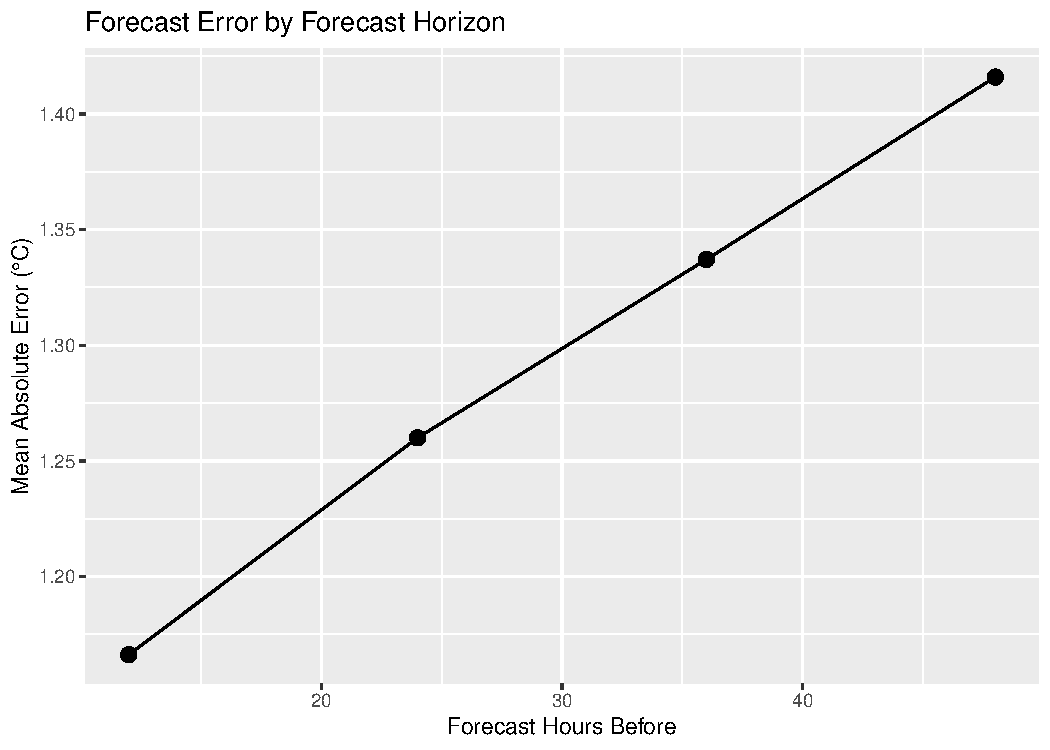
\includegraphics[keepaspectratio]{Course-project_files/figure-pdf/unnamed-chunk-3-1.pdf}}

The mean error for all forecast horizons is negative. This indicates
that, on average, forecasts underestimate the actual temperature. The
mean error is surprisingly slightly lower for forecasts made 48 hours in
advance rather than 12 hours before, while the standard deviation
increases as the hours before the observation increase.

\subsubsection{Climate zones}\label{climate-zones}

The dataset is based on the Köppen climate classification, a system
developed by German climatologist Wladimir Köppen to describe climates
depending on local vegetation by using letters. These letters indicate
various things in order: climate type, precipitation and temperature.

Here is a map of the world showing the 5 climate types:
\pandocbounded{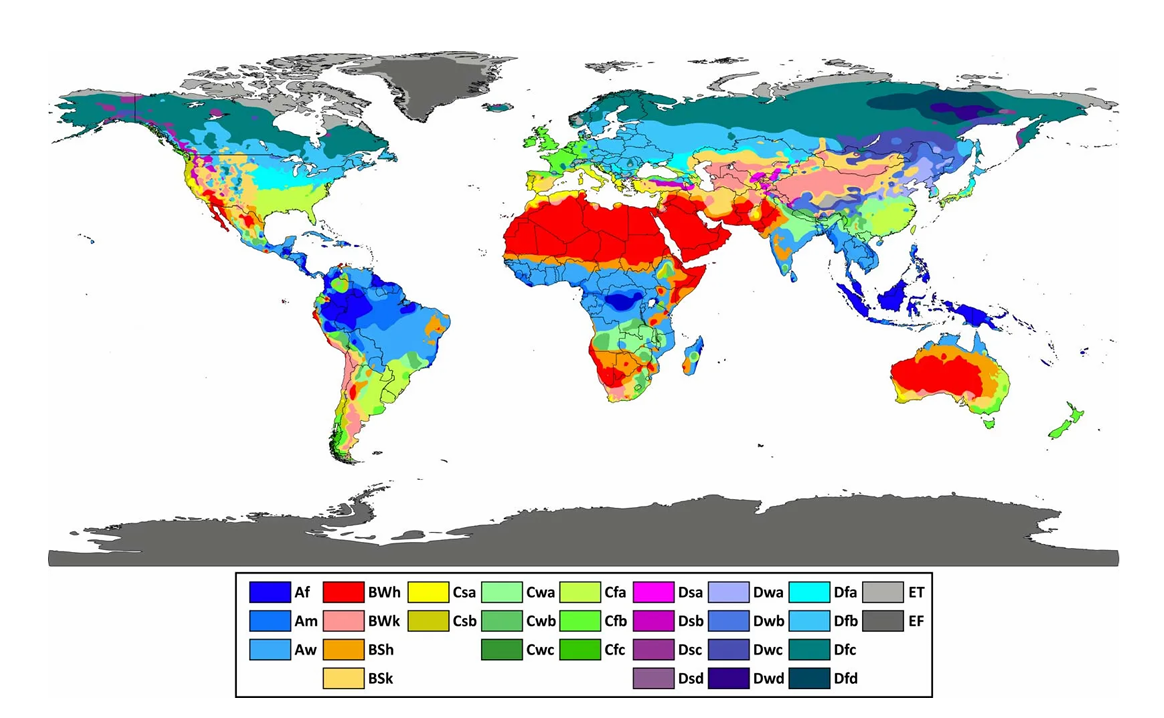
\includegraphics[keepaspectratio]{koppenmap_.png}}

Source:
\href{https://www.britannica.com/science/Koppen-climate-classification\#/media/1/322068/206711}{Encyclopædia
Britannica} -- M.C. Peel, B.L. Finlayson, and T.A. McMahon (2007).

Are some climate zones harder to predict than others? Since in the data
there are 15 climates included and some present more observations than
others, we decided to study only the top 7.

\begin{Shaded}
\begin{Highlighting}[]
\NormalTok{summary\_koppen\_error }\OtherTok{\textless{}{-}}\NormalTok{ weather\_forecast\_accuracy}\SpecialCharTok{|\textgreater{}}
  \FunctionTok{group\_by}\NormalTok{(koppen) }\SpecialCharTok{|\textgreater{}}
  \FunctionTok{summarise}\NormalTok{(}\AttributeTok{n =} \FunctionTok{n}\NormalTok{(),}
    \AttributeTok{mean\_error =} \FunctionTok{mean}\NormalTok{(forecast\_temp\_c}\SpecialCharTok{{-}}\NormalTok{observed\_temp\_c),}
    \AttributeTok{median\_error =} \FunctionTok{median}\NormalTok{(forecast\_temp\_c}\SpecialCharTok{{-}}\NormalTok{observed\_temp\_c),}
    \AttributeTok{mean\_sd =} \FunctionTok{sd}\NormalTok{(forecast\_temp\_c}\SpecialCharTok{{-}}\NormalTok{observed\_temp\_c)) }\SpecialCharTok{|\textgreater{}}
  \FunctionTok{filter}\NormalTok{(n }\SpecialCharTok{\textgreater{}} \DecValTok{10000}\NormalTok{) }\SpecialCharTok{|\textgreater{}}
  \FunctionTok{arrange}\NormalTok{(mean\_error) }

\NormalTok{summary\_koppen\_error}
\end{Highlighting}
\end{Shaded}

\begin{verbatim}
# A tibble: 7 x 5
  koppen      n mean_error median_error mean_sd
  <chr>   <int>      <dbl>        <dbl>   <dbl>
1 Dfc     10349     -0.746       -0.556    2.24
2 BSk     61833     -0.409       -0.556    1.99
3 Csb     58585     -0.341       -0.556    1.68
4 Dfb     96055     -0.258        0        1.80
5 Cfb     17209     -0.213        0        1.62
6 Dfa     79199     -0.196        0        1.77
7 Cfa    269295     -0.141        0        1.65
\end{verbatim}

\pandocbounded{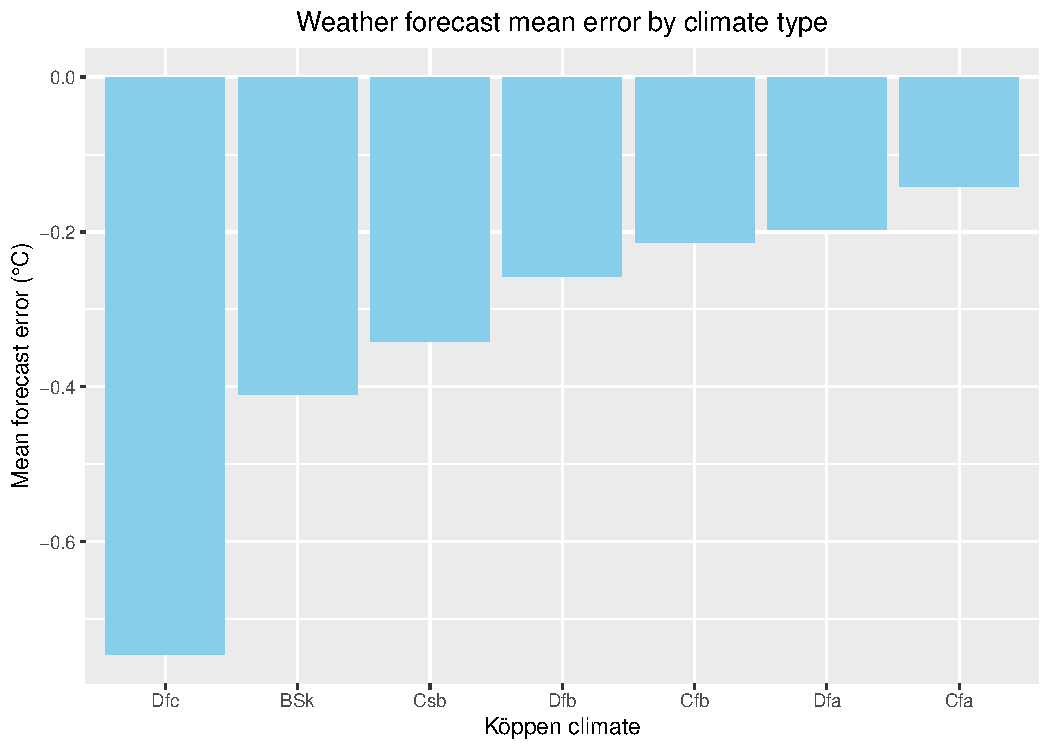
\includegraphics[keepaspectratio]{Course-project_files/figure-pdf/unnamed-chunk-5-1.pdf}}

Forecast errors are highest for Dfc (Subarctic) climate, which is a type
of climate with no significant difference in precipitations between
seasons, followed by the BSk (Arid Steppe) Climate, characterized by low
precipitation and large temperature ranges.

\subsubsection{Seasonal Forecast
Accuracy}\label{seasonal-forecast-accuracy}

Do seasons influence weather forecast accuracy?

\begin{Shaded}
\begin{Highlighting}[]
\FunctionTok{ggplot}\NormalTok{(season\_summary, }\FunctionTok{aes}\NormalTok{(}\AttributeTok{x =} \FunctionTok{factor}\NormalTok{(season, }\AttributeTok{levels =} \FunctionTok{c}\NormalTok{(}\StringTok{"Fall"}\NormalTok{,}\StringTok{"Winter"}\NormalTok{,}\StringTok{"Spring"}\NormalTok{,}\StringTok{"Summer"}\NormalTok{)),}
    \AttributeTok{y =} \FunctionTok{factor}\NormalTok{(forecast\_hours\_before),}
    \AttributeTok{fill =}\NormalTok{ mean\_error)) }\SpecialCharTok{+}
  \FunctionTok{geom\_tile}\NormalTok{(}\AttributeTok{color =} \StringTok{"white"}\NormalTok{) }\SpecialCharTok{+}
  \FunctionTok{scale\_fill\_gradient}\NormalTok{(}\AttributeTok{low =} \StringTok{"white"}\NormalTok{, }\AttributeTok{high =} \StringTok{"darkgreen"}\NormalTok{) }\SpecialCharTok{+}
  \FunctionTok{labs}\NormalTok{(}
    \AttributeTok{title =} \StringTok{"Forecast Error by Season and Forecast Horizon"}\NormalTok{,}
    \AttributeTok{x =} \StringTok{"Season"}\NormalTok{,}
    \AttributeTok{y =} \StringTok{"Forecast Hours Before"}\NormalTok{,}
    \AttributeTok{fill =} \StringTok{"Mean Error (°C)"}
\NormalTok{  ) }\SpecialCharTok{+}
  \FunctionTok{theme\_minimal}\NormalTok{() }\SpecialCharTok{+}
  \FunctionTok{theme}\NormalTok{(}
    \AttributeTok{plot.title =} \FunctionTok{element\_text}\NormalTok{(}\AttributeTok{hjust =} \FloatTok{0.5}\NormalTok{)}
\NormalTok{  )}
\end{Highlighting}
\end{Shaded}

\pandocbounded{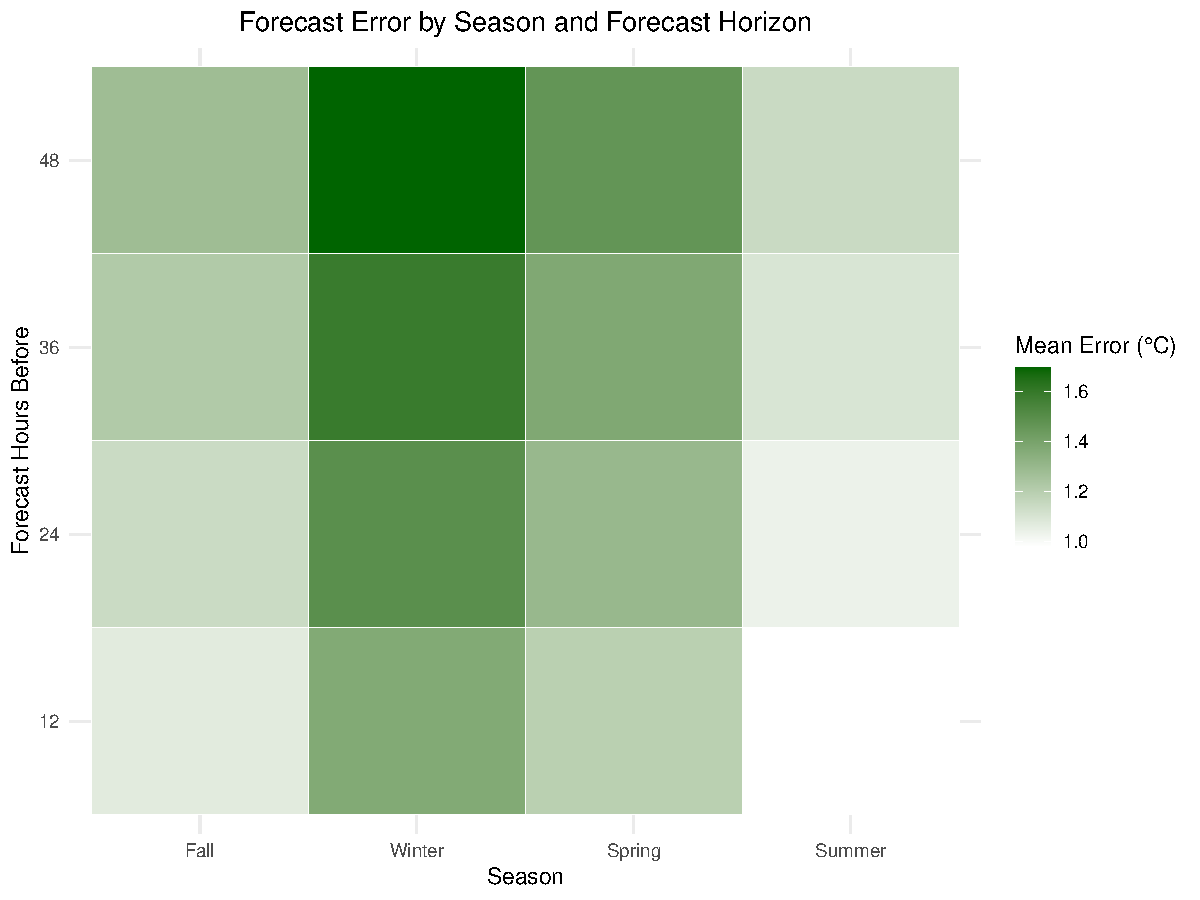
\includegraphics[keepaspectratio]{Course-project_files/figure-pdf/unnamed-chunk-7-1.pdf}}

The heatmap clearly shows that weather accuracy is particularly low in
Winter. This can be attributed to different factors, such as pressure
systems and movement of the Arctic Air. To learn more about the reasons,
read this article written by David M. Ewalt for the
\href{https://www.scientificamerican.com/article/why-are-winter-storm-forecasts-all-over-the-place/}{\emph{Scientific
American}}, focused on US weather forecasts, or this blog post from
\href{https://www.severe-weather.eu/long-range-2/winter-season-forecast-accuracy-snow-temperature-pressure-united-states-europe-verification-fa/}{\emph{Severe
Weather Europe}} for an in-depth worldwide perspective of the
phenomenon.

\subsubsection{Elevation Change}\label{elevation-change}

Elevation change refers to the difference in elevation between two
points on Earth's surface (typically relative to sea level). The dataset
presents two columns related to elevation:
\texttt{elevation\_change\_four} and \texttt{elevation\_change\_eight}.
We decided to use the latter because it's considered more reliable and
accurate due to the incorporation of more data points, reducing
directional bias and improving representation of local topography.

\begin{verbatim}
# A tibble: 158 x 4
   city           elevation elevation_error elevation_sd
   <chr>              <dbl>           <dbl>        <dbl>
 1 KEY_WEST            0.46          0.0622         1.08
 2 W_PALM_BEACH        1.65          0.618          1.36
 3 MIAMI_BEACH         2.55          0.518          1.05
 4 NEW_ORLEANS         2.82          0.529          1.48
 5 SAVANNAH            4.63          0.0863         1.50
 6 FARGO               5.49          0.0524         1.98
 7 LAKE_CHARLES        5.52          0.0958         1.57
 8 BROWNSVILLE         8.96          0.232          1.62
 9 DAYTONA_BEACH       9.68          0.132          1.40
10 CORPUS_CHRISTI     13.4           0.131          1.78
# i 148 more rows
\end{verbatim}

\begin{Shaded}
\begin{Highlighting}[]
\NormalTok{weather\_forecast\_accuracy}\SpecialCharTok{|\textgreater{}}
  \FunctionTok{group\_by}\NormalTok{(city) }\SpecialCharTok{|\textgreater{}}
  \FunctionTok{summarise}\NormalTok{(}
  \AttributeTok{elevation\_error =} \FunctionTok{abs}\NormalTok{(}\FunctionTok{mean}\NormalTok{(forecast\_temp\_c }\SpecialCharTok{{-}}\NormalTok{ observed\_temp\_c)),}
  \AttributeTok{elevation\_change\_eight =} \FunctionTok{mean}\NormalTok{(elevation\_change\_eight)}
\NormalTok{  ) }\SpecialCharTok{|\textgreater{}}
  \FunctionTok{ggplot}\NormalTok{(}\AttributeTok{mapping=}\FunctionTok{aes}\NormalTok{(}\AttributeTok{x =}\NormalTok{ elevation\_change\_eight, }\AttributeTok{y =}\NormalTok{ elevation\_error)) }\SpecialCharTok{+}
  \FunctionTok{geom\_point}\NormalTok{(}\AttributeTok{colour =} \StringTok{"blue"}\NormalTok{, }\AttributeTok{alpha =} \FloatTok{0.5}\NormalTok{) }\SpecialCharTok{+}
  \FunctionTok{geom\_smooth}\NormalTok{(}\AttributeTok{method =} \StringTok{"loess"}\NormalTok{, }\AttributeTok{colour =} \StringTok{\textquotesingle{}pink\textquotesingle{}}\NormalTok{) }\SpecialCharTok{+}
  \FunctionTok{labs}\NormalTok{(}\AttributeTok{x =} \StringTok{"Elevation Change Eight"}\NormalTok{,}
  \AttributeTok{y =} \StringTok{"Mean error"}\NormalTok{,}
  \AttributeTok{title =} \StringTok{"Forecast Error by Elevation Change Eight"}\NormalTok{) }\SpecialCharTok{+}
   \FunctionTok{theme}\NormalTok{(}
    \AttributeTok{plot.title =} \FunctionTok{element\_text}\NormalTok{(}\AttributeTok{hjust =} \FloatTok{0.5}\NormalTok{)}
\NormalTok{  )}
\end{Highlighting}
\end{Shaded}

\pandocbounded{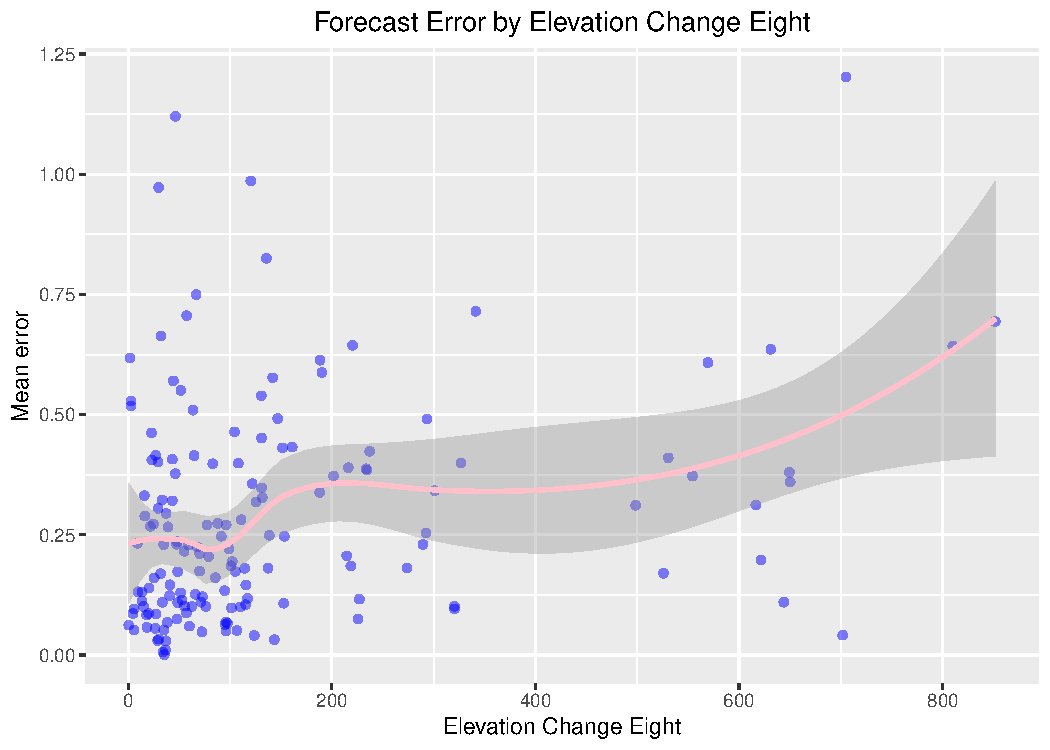
\includegraphics[keepaspectratio]{Course-project_files/figure-pdf/unnamed-chunk-9-1.pdf}}

The plot suggests a slight increase in forecast error with elevation.

\begin{quote}
``Differing amounts and types of air molecules present in atmosphere's
layers result in temperatures that cool with height at some altitudes
and warm with height at others.''\footnote{UCAR - Center for Science
  Education. \emph{Change in the Atmosphere with Altitude.}
  https://scied.ucar.edu/learning-zone/atmosphere/change-atmosphere-altitude
  (Accessed March 9, 2026)}
\end{quote}

\subsubsection{Conclusions}\label{conclusions}

This report shows that weather forecasts are pretty accurate with a mean
error between 0.21°C and 0.26°C depending on the hours the forecast was
made before the observed temperature. Variables that affect accuracy are
climate zones, seasonality and elevation above sea level. Further
studies could be carried out on geographic and local factors and
long-term analysis across decades to see if there is an improvement in
employed models.




\end{document}
